\begin{frame}{Circulation du discours médical au prisme du numérique}
\centering
Objectif : aborder computationnellement la question des circulations des phénomènes textuels complexes.
\begin{figure}
    \centering
    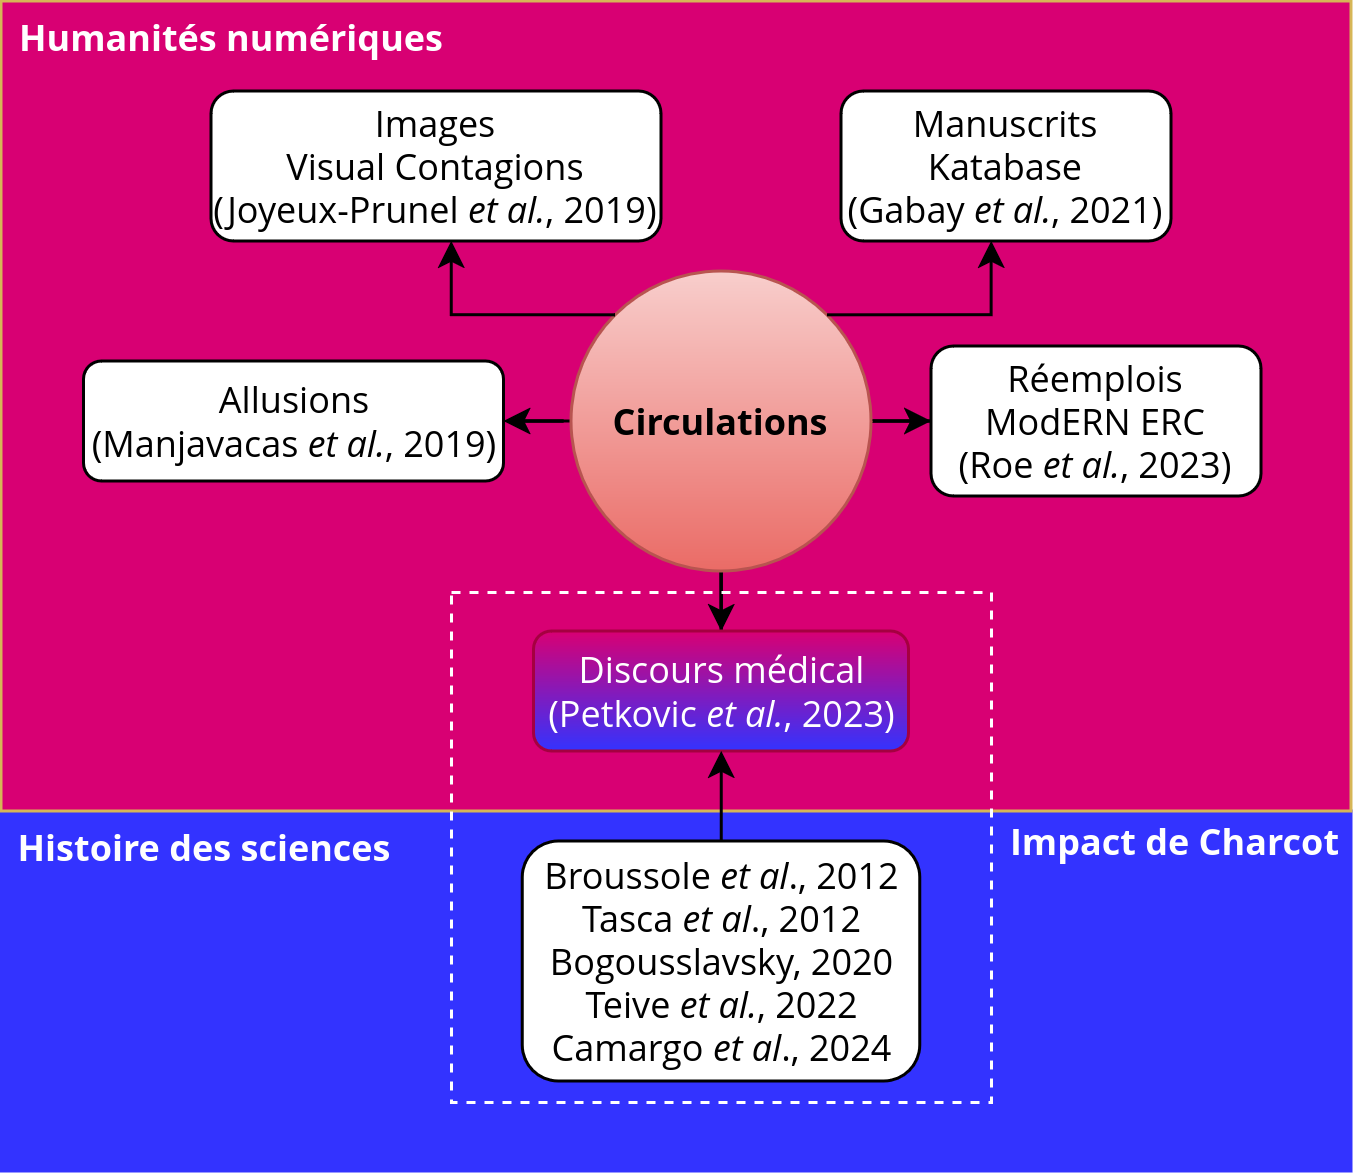
\includegraphics[width=65mm,scale=0.5]{pic/dh_histoire-sciences.png}
    \caption{Études (numériques) des circulations des savoirs.}
    \label{fig:enter-label}
\end{figure}
\notecite{joyeux2019visual}
\notecite{gabay2021katabase}
\notecite{manjavacas2019}
\notecite{tasca2012women}
\notecite{bogousslavsky2020}
\notecite{teive2022thomas}
\nocite{camargo2024}
% Influence de Charcot : \cite{bogousslavsky}, \cite{camargo}
% Constitution et exploitation de ce fonds au prisme du numérique
\end{frame}

